\documentclass[a4paper]{article}
\usepackage[top=2cm, bottom=2cm, left=2cm, right=2cm]{geometry}

\usepackage{color}
\usepackage{graphicx}
\usepackage{float}
\usepackage{framed}

\usepackage{mathtools}
\usepackage{amssymb}
\usepackage{algorithmic}

\usepackage{hyperref}
\hypersetup{
    colorlinks=true,
    linkcolor=black,
    filecolor=cyan,
    urlcolor=magenta,
}

\usepackage{listings}
\definecolor{comment_colour}{rgb}{0,0.6,0}
\definecolor{number_colour}{rgb}{0.5,0.5,0.5}
\definecolor{string_colour}{rgb}{0.58,0,0.82}
\lstset{
    frame=single,
    numbers=left,
    breaklines=true,
    breakatwhitespace=true,
    commentstyle=\color{comment_colour},
    keywordstyle=\color{blue},
    numberstyle=\tiny\color{number_colour},
    stringstyle=\color{string_colour}
}

\title{QLearningAgent Pseudo-code}
\date{\today}
\author{Hugo McNally}

\begin{document}
\large
\section*{Q-learning Agent Pseudo-code}

The Q-learning algorithm was taken from page 131 of the second edition of
'Reinforcement Learning: An Introduction'
by Richard S. Sutton and Andrew G. Barto,
which can be found at \url{http://incompleteideas.net/book/the-book.html}
and which is shown below in Figure~\ref{orig}.
I have also rewritten this algorithm in Figure~\ref{orig-re}
so that my changes are a little easier to follow.

\begin{figure}[H]
\begin{center}
    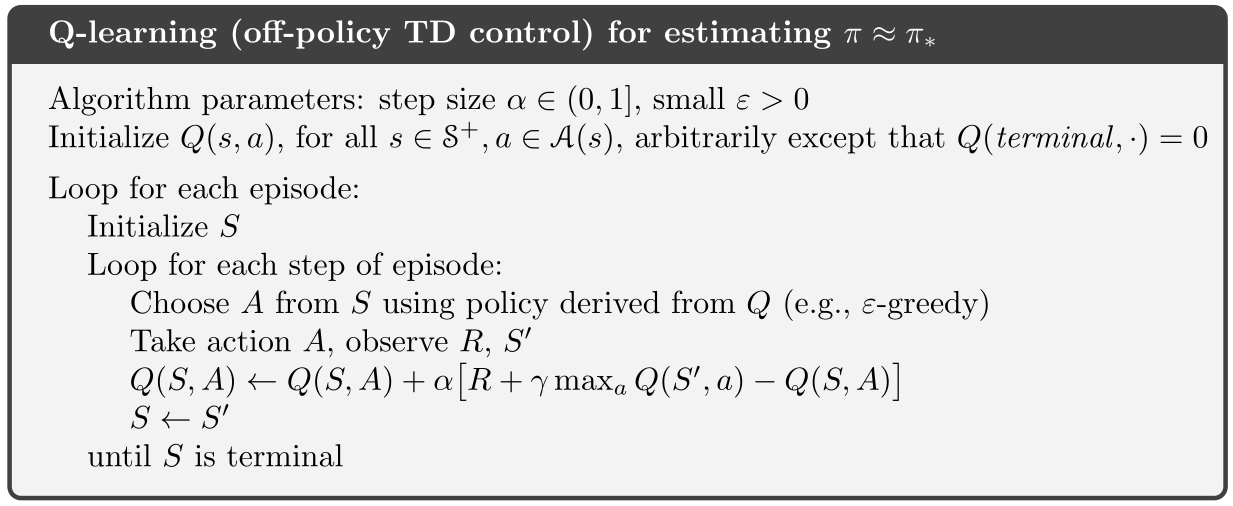
\includegraphics[width=30em]{Q-learning_algorithm.png}
\end{center}
\caption{The original Q-learning algorithm.}
\label{orig}
\end{figure}

\begin{figure}[H]
\begin{framed}
\begin{algorithmic}[1]
    \REQUIRE $\alpha \in (0, 1]$ and $\epsilon > 0$
    \STATE $Q(s, a) \gets 0, \quad\forall s, a$
    \FORALL{episodes}
    \STATE $S \gets$ starting state
    \REPEAT
    \STATE $A \gets \epsilon$-greedy choice from $Q(S, \cdot)$
    \STATE Take action $A$, observe $R, S'$
    \STATE $Q(S, A) \leftarrow Q(S, A)
    + \alpha [R + \gamma \max_a Q(S', a) - Q(S, A)]$
    \STATE $S \gets S'$
    \UNTIL{$S$ is terminal}
    \ENDFOR
\end{algorithmic}
\end{framed}
\caption{The original Q-learning algorithm rewritten.}
\label{orig-re}
\end{figure}

With the agent learning from the experiences (transitions)
of a number of nodes in a graph,
another loop needs to be added to iterate though each node of the graph.
Because the next state of a node and its next best action
can be dependant on the state of its neighbours,
the action of each node should be carried out together
before learning from any of these actions.
Currently, this is achieved with two loops as shown in Figure~\ref{my}.
In the first loop (line 6),
an action is selected for each node.
Then all the actions are performed (line 9).
After this,
the second loop (line 10) learns from the transitions
which resulted from each node's action.

\begin{figure}[H]
\begin{framed}
\begin{algorithmic}[1]
    \REQUIRE Learning rate: $\alpha \in (0, 1]$
    and discount factor: $\gamma \in (0, 1]$
    \STATE $Q(s, a) \gets 0, \quad\forall s, a$
    \STATE $G$ is a graph of $N$ nodes
    \FORALL{episodes}
    \STATE $S^t \gets$ the $N$ starting states of the nodes
    \FOR{$t = 0$ \TO deadline}
    \FORALL{$n \in G$}
    \STATE $A^t_n \gets \epsilon$-greedy choice from $Q(S^t_n, \cdot)$
    \ENDFOR
    \STATE Find $S^{t+1}$, $R^t$ from $S^t$, $A^t$, $G$
    \FORALL{$n \in G$}
    \STATE $Q(S^t_n, A^t_n) \leftarrow Q(S^t_n, A^t_n)
    + \alpha [R^t + \gamma \max_a Q(S^{t+1}_n, a) - Q(S^t_n, A^t_n)]$
    \ENDFOR
    \ENDFOR
    \ENDFOR
\end{algorithmic}
\end{framed}
\caption{The adapted Q-learning algorithm.}
\label{my}
\end{figure}

The code for the main training loop is shown in Figure~\ref{code-main}.
Lines 6, 9 and 10 of Figure~\ref{my} corresponds to lines 7, 17 and 20
of Figure~\ref{code-main} respectively.
Action selection is performed by the \texttt{QLearningAgent}'s
\texttt{choose\_epsilon\_greedy\_action} method shown in Figure~\ref{code-eps}.
At the moment the node's state is made up of only
the time step and the node's normalised fitness
(the fitness after being normalised but before the monotonic function),
which is why these are the two values passed to the method.

The environment's \texttt{run\_time\_step} performs the set action
for each node and finally the agent learns from each node's experience
using its \texttt{learn} method.
This method is passed the time step and node's normalised fitness before
and after the transition,
as well as the action which it took and fitness resulting from this action
(this is after the monotonic function).
This fitness is used as a reward in the final time step.
The code for this method is shown in Figure~\ref{code-learn}.
This \texttt{learn} method calls a private \texttt{\_update\_q\_table}
calculates the equation on line 11 of the pseudo-code in Figure~\ref{my}.

\begin{figure}[H]
\lstinputlisting[
    language=python,
    linerange={58-94}
]{../../train.py}
\caption{The main training loop from train.py (lines 58 -- 94).}
\label{code-main}
\end{figure}


\begin{figure}[H]
\lstinputlisting[
    language=python,
    linerange={76-88}
]{../../agents/qlearning.py}
\caption{
    QLearningAgent.choose\_epsilon\_greedy\_action
    from agents/qlearning.py (lines 76 -- 88).
}
\label{code-eps}
\end{figure}

\begin{figure}[H]
\lstinputlisting[
    language=python,
    linerange={94-106}
]{../../agents/qlearning.py}
\caption{
    QLearningAgent.learn
    from agents/qlearning.py (lines 94 -- 106).
}
\label{code-learn}
\end{figure}

\begin{figure}[H]
\lstinputlisting[
    language=python,
    linerange={58-69}
]{../../agents/qlearning.py}
\caption{
    QLearningAgent.\_update\_q\_table
    from agents/qlearning.py (lines 58 -- 69).
}
\label{code-update}
\end{figure}

\end{document}
